13. \begin{figure}[ht!]
\center{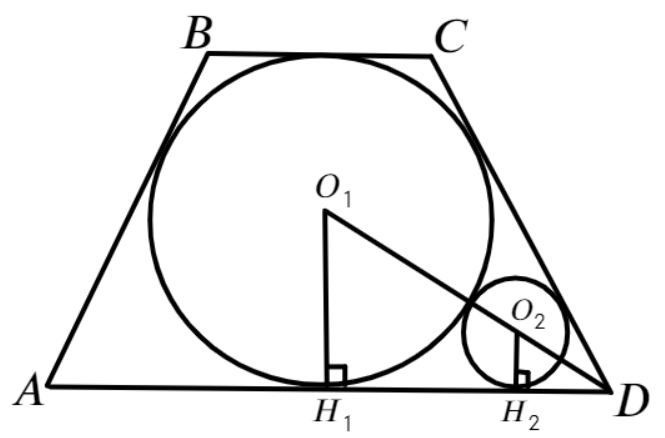
\includegraphics[scale=0.35]{g9-13.png}}
\end{figure}\\
Так как трапеция является описанной, $AB+CD=BC+AD,\ 2AB=2+8=10,\ AB=5.$ Опустив две высоты из вершин $B$ и $C,$ можно найти высоту трапеции: $h=\sqrt{5^2-\left(\cfrac{8-2}{2}
ight)^2}=4.$ Тогда радиус большей окружности равен $4:2=2.$ Раз обе окружности касаются сторон $AD$ и $CD,$ их центры лежат на биссектрисе угла $D.$ Проведём перпендикуляры $O_1H_1$ и $O_2H_2$ к точкам касания. Найдём $O_1D=\sqrt{4^2+2^2}=2\sqrt{5}.$ Пусть радиус меньшей окружности равен $x,$ тогда  $O_2D=2\sqrt{5}-2-x.$ Из подобия треугольников $O_1H_1D$ и $O_2H_2D$ (по двум углам) получаем соотношение $\cfrac{2\sqrt{5}-2-x }{2\sqrt{5}}=\cfrac{x}{2},$ откуда $4\sqrt{5}-4-2x=2\sqrt{5}x,\ 2x(1+\sqrt{5})=4(\sqrt{5}-1),\ x=\cfrac{2(\sqrt{5}-1)}{1+\sqrt{5}}=3-\sqrt{5}.$\\
